\documentclass[headheight=4.5cm,
			   margin=2cm,
			   titlewidth=0.6,
			   sansserif,
			   firstcolor=color1,
			   secondcolor=color2,
			   logo=myLogo.png,
			   % footband=myFootBand.png
			  ]{TelecomNancy}

\definecolor{color1}{RGB}{100, 100, 100}
\definecolor{color2}{RGB}{220, 0, 0}
\usepackage{amsmath}
\usepackage{amssymb}
\usepackage{pifont}
\usepackage{tikz}
\usepackage{tabularx}
\usepackage{array}
\usepackage{booktabs}
\usepackage{multirow}
\usepackage{tabu}
\usepackage[UTF8]{ctex}

\begin{document}

	\coursetitle{三角函数 知识清单}
	\courselevel{高中数学一年级}
	\courseyear{2017.12.20}
	
	% \globalinstructions[填空前的提示]
	% {
	% 	 在填这个空之前,希望大家能借助这次机会,将基本的知识性概念再熟络于心,千万不要忽视基础的威力,数学本身就是一门基础的学科,但是数学的影响力却非常物所能及. 
	% }

	\nextExercise[角的概念的推广——任意角]{
		角的概念:平面内一条\underline{\hspace{1cm}}绕着\underline{\hspace{1cm}}从一个位置\underline{\hspace{1cm}}到另一个位置所形成的图形.
	}
		\begin{minipage}{0.7\textwidth}
			\nextQuestion{如图,OA 为角$\alpha$的\underline{\hspace{1cm}},OB 为角$\alpha$的\underline{\hspace{1cm}}.}

			\nextQuestion{正角:按\underline{\hspace{1.5cm}}方向旋转形成的角;\\负角:按\underline{\hspace{1.5cm}}方向旋转形成的角;\\零角:射线没有作\underline{\hspace{1.5cm}}形成一个零角.}
		\end{minipage}
		\begin{minipage}{0.3\textwidth}
			\begin{tikzpicture}
    			\draw (0,0)node[left]{$O$}--(1.414,0)node[right]{$A$};
    			\draw (0,0)--(1,1)node[above]{$B$};
    			\draw[very thin] (0.25,0) arc (0:45:0.25) node[right]{$\alpha$};
  			\end{tikzpicture}
		\end{minipage}
 
		\nextInstructions{
			终边相同的角:所有与角$\alpha$终边相同的角,连同角$\alpha$在内,可构成一个集合:$S=\underline{\hspace{3cm}}$.
		}

		\nextQuestion{轴线角的表示:\\
		\ding{172} 终边在$x$轴正半轴的所有角组成的集合:\underline{$\{\alpha|\alpha=2k\pi, k\in \mathbf{Z}\}$};\\
		\ding{173} 终边在$y$轴正半轴的所有角组成的集合:\underline{\hspace{4cm}};\\
		\ding{174} 终边在$x$轴负半轴的所有角组成的集合:\underline{\hspace{4cm}};\\
		\ding{175} 终边在$y$轴负半轴的所有角组成的集合:\underline{\hspace{4cm}};\\
		\ding{176} 终边在$x$轴上的所有角组成的集合:\underline{\hspace{4cm}};\\
		\ding{177} 终边在$y$轴上的所有角组成的集合:\underline{\hspace{4cm}};\\
		\ding{178} 终边在坐标轴上的所有角组成的集合:\underline{\hspace{4cm}};\\
		}

		\nextQuestion{象限角的表示:\\
		\ding{172} 终边在第一象限的角的所属范围:\underline{$(2k\pi,\frac{\pi}{2}+2k\pi),k\in\mathbf{Z}$};\\
		\ding{173} 终边在第二象限的角的所属范围:\underline{\hspace{4cm}};\\
		\ding{174} 终边在第三象限的角的所属范围:\underline{\hspace{4cm}};\\
		\ding{175} 终边在第四象限的角的所属范围:\underline{\hspace{4cm}} 或 \underline{$(-\frac{\pi}{2}+2k\pi,2k\pi),k\in\mathbf{Z}$}.\\
		}

	\nextExercise[弧度制]{将长度等于\underline{\hspace{1cm}}长的弧 所对的圆心角 叫$1$弧度的角,记作\underline{\hspace{1cm}}.(弧度单位rad一般省略不写)\\
	这种用\underline{\hspace{1cm}}作单位来度量角的单位制称为弧度制.}
	\begin{minipage}{0.7\textwidth}
		\nextQuestion{角度、弧度的换算:\\
		$\pi=180^\circ \quad 1=\underline{\hspace{1cm}} \quad 1^\circ=\underline{\hspace{1cm}}$
		}
		\nextQuestion{弧长公式:\\
		$l=\underline{\hspace{1cm}}$ $\quad$ (等价推广:$r=\underline{\hspace{1cm}} \quad |\alpha|=\underline{\hspace{1cm}}$.)
		}
		\nextQuestion{扇形面积公式:\\
		$S=\underline{\hspace{1.5cm}}=\underline{\hspace{1.5cm}}=\underline{\hspace{1.5cm}}$\\
		(其中$r$为圆的半径,$\alpha$为圆心角的弧度数,$l$为弧长,$S$为扇形面积)
		}
	\end{minipage}
	\begin{minipage}{0.3\textwidth}
		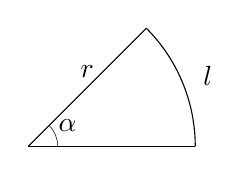
\begin{tikzpicture}[scale=1.5]
			\draw (0,0) -- (1.414,0);
			\draw (0,0) --node[above]{$r$} (1,1);
			\draw[very thin] (0.25,0) arc (0:45:.25) node[right]{$\alpha$};
			\draw (1.414,0) arc (0:45:1.414) (1.4,0.6)node[right]{$l$};
		\end{tikzpicture}
	\end{minipage}


% ================== 第二天知识清单=================
	\newpage

	\nextExercise[任意角的三角函数]{}

		\nextQuestion{任意角三角函数的定义:\\
		\emph{定义一:}(借助\textbf{单位圆}来定义)\\
		如图,设$\alpha$为一个任意角,它的终边与单位圆交于$P(x,y)$, 则:\\
		\begin{minipage}{0.6\textwidth}
			\ding{172} $y$叫做$\alpha$的\underline{\hspace{1cm}},记作 \underline{$\sin\alpha=y$};\\
			\ding{173} $x$叫做$\alpha$的\underline{\hspace{1cm}},记作\underline{\hspace{1.5cm}};\\
			\ding{174} $\frac{y}{x}$叫做$\alpha$的\underline{\hspace{1cm}},记作\underline{\hspace{1.5cm}};\\
		\end{minipage}
		\begin{minipage}{0.4\textwidth}
			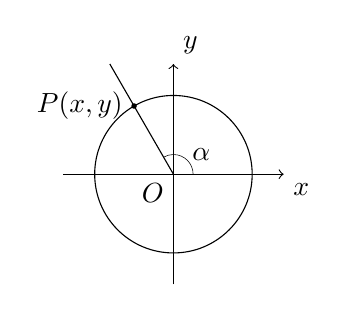
\begin{tikzpicture}
				\draw[->] (-1.4,0) -- (1.4,0) node[anchor=north west]{$x$};
				\draw[->] (0,-1.4) -- (0,1.4) node[anchor=south west]{$y$};
				\draw (0,0) node[anchor=north east]{$O$};
				\draw (0,0) circle(1);
				\draw (0,0) -- (-0.808,1.4) (-0.52,0.866)node[left]{$P(x,y)$};
				\fill (-0.5,0.866) circle [radius=1pt];
				\draw[very thin] (0.25,0) arc (0:120:.25) (.12,.25)node[right]{$\alpha$};
			\end{tikzpicture}
		\end{minipage}

		\emph{定义二:}(不再限定必须在单位圆内)\\
		如图,设$\alpha$为一个任意角,在$\alpha$的终边上任取一点$P(x,y)$(但$P$不能为原点),则:\\
		\begin{minipage}{0.6\textwidth}
		$r=|OP|=\underline{\hspace{2cm}}$\\
		$\sin\alpha=\underline{\, \frac{y}{r}\, } \quad \cos\alpha=\underline{\hspace{1cm}} \quad \tan\alpha=\underline{\hspace{1cm}}.$
		\end{minipage}
		\begin{minipage}{0.4\textwidth}
			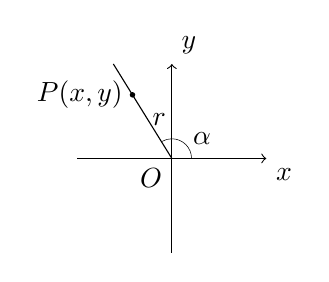
\begin{tikzpicture}
				\draw[->] (-1.2,0) -- (1.2,0) node[anchor=north west]{$x$};
				\draw[->] (0,-1.2) -- (0,1.2) node[anchor=south west]{$y$};
				\draw (0,0) node[anchor=north east]{$O$};
				\draw (0,0) -- (-0.743,1.2) (-.37,.5)node[right]{$r$};
				\fill (-0.5,0.808) circle [radius=1pt] node[left]{$P(x,y)$};
				\draw[very thin] (.25,0) arc (0:120:.25) (.15,.25)node[right]{$\alpha$};
			\end{tikzpicture}
		\end{minipage}
		}
		

		\nextQuestion{正弦、余弦、正切函数值 在各象限的符号问题:\\
		请仿照$\sin \alpha$在各坐标轴以及在各象限的符号情况,写出$\cos \alpha$及$\tan \alpha$的符号情况.\\
		\begin{minipage}{0.3\textwidth}
			\begin{tikzpicture}
				\draw[->] (-1.2,0) node[left]{$0$} -- (1.2,0) node[right]{$0$};
				\draw[->] (0,-1.2) node[below]{$-1$} node[below=10pt]{$\sin \alpha$} -- (0,1.2) node[above]{$1$};
				\draw (0,0) node[anchor=south west]{$+$} node[anchor=south east]{$+$} node[anchor=north east]{$-$} node[anchor=north west]{$-$};
			\end{tikzpicture}
		\end{minipage}
		\begin{minipage}{0.3\textwidth}
			\begin{tikzpicture}
				\draw[->] (-1.2,0) -- (1.2,0);
				\draw[->] (0,-1.2) node[below=10pt]{$\cos \alpha$} -- (0,1.2);
			\end{tikzpicture}
		\end{minipage}
		\begin{minipage}{0.3\textwidth}
			\begin{tikzpicture}
				\draw[->] (-1.2,0) -- (1.2,0);
				\draw[->] (0,-1.2) node[below=10pt]{$\tan \alpha$} -- (0,1.2);
			\end{tikzpicture}
		\end{minipage}

		}

		\nextQuestion{常用特殊角 三角函数值表:\\
		\begin{tabular}{c|c|c|c|c|c|c|c|c|c}
		\hline
		角$\alpha$ & $\phantom{1}0^\circ\phantom{1}$ & $\phantom{1}30^\circ$ & $\phantom{1}45^\circ$ & $\phantom{1}60^\circ$ & $\phantom{1}90^\circ$ & $120^\circ$ & $150^\circ$ & $180^\circ$ & $270^\circ$\\
		\hline
		角$\alpha$的弧度数 & $\quad$ & $\quad$ & $\quad$ & $\quad$ & $\quad$ & $\quad$ & $\quad$ & $\quad$ & $\quad$\\
		\hline
		$\sin\alpha$ & $\quad$ & $\quad$ & $\quad$ & $\quad$ & $\quad$ & $\quad$ & $\quad$ & $\quad$ & $\quad$\\
		\hline
		$\cos\alpha$ & $\quad$ & $\quad$ & $\quad$ & $\quad$ & $\quad$ & $\quad$ & $\quad$ & $\quad$ & $\quad$\\
		\hline
		$\tan\alpha$ & $\quad$ & $\quad$ & $\quad$ & $\quad$ & $\quad$ & $\quad$ & $\quad$ & $\quad$ & $\quad$\\
		\hline

		\end{tabular}
		}

		\nextQuestion{同角三角函数的基本关系式:\\
		$\sin^2\alpha+\cos^2\alpha=\underline{\hspace{0.5cm}} \quad \tan\alpha=\underline{\hspace{1cm}}$
		}

% ================= 第三天知识清单 ==============

	\newpage

	\nextExercise[诱导公式]{口诀:“\textbf{奇变偶不变,符号看象限}”.\\
	\ding{172} “奇”“偶”指“$\frac{\pi}{2}$”的奇数倍和偶数倍;\\
	\ding{173} “变”与“不变”是指函数名称是否改变;\\
	\ding{174} 把$\alpha$ 当作锐角 $\longrightarrow$ 找象限 $\longrightarrow$ 判断符号.
	}

		\begin{tabularx}{0.9\textwidth}{c|X|X|X|X|X|X|X|X|X}
			\hline
			 & $2k\pi+\alpha$ & $2\pi+\alpha$ & $\phantom{2}\pi+\alpha$ & $\phantom{2}\pi-\alpha$ & $\phantom{2}-\alpha$ & $\phantom{2}\frac{\pi}{2}-\alpha$ & $\phantom{2}\frac{\pi}{2}+\alpha$ & $\frac{3\pi}{2}-\alpha$ & $\frac{3\pi}{2}+\alpha$\\
			\hline
			$\sin$ & & & & & & & & & \\
			\hline
			$\cos$ & & & & & & & & & \\
			\hline
			$\tan$ & & & & & & & & & \\
			\hline
		\end{tabularx}

	\nextExercise[基础三角函数的图象与性质]{}

		\begin{tabular}[c]{l|p{4.5cm}<{\centering}|p{4.5cm}<{\centering}|p{4.5cm}<{\centering}}
			\hline
			 & $f(x)=\sin x$ & $f(x)=\cos x$ & $f(x)=\tan x$\\
			\hline
			\multirow{5}{*}{\ding{172} 列表} & & & \\
			 & & & \\
			 & & & \\
			 & & & \\
			 & & & \\
			\hline
			\multirow{6}{*}{\ding{173} 图象} & & & \\
			 & & & \\
			 & & & \\
			 & & & \\
			 & & & \\
			 & & & \\
			\hline
			\ding{174} 定义域 & & & \\
			\hline
			\ding{175} 值域 & & & \\
			\hline
			\ding{176} 周期 & & & \\
			\hline
			\multirow{3}{*}{\ding{177} 单调性} & & & \\
			 & & & \\
			 & & & \\
			\hline
			\multirow{3}{*}{\ding{178} 最值} & & & \\
			 & & & \\
			 & & & \\
			\hline
			\ding{179} 奇偶性 & & & \\
			\hline
			\multirow{2}{*}{\ding{180} 对称性} & 对称中心:$(k\pi,0)\phantom{12345678}$ & & \\
			 & 对称轴:$x=\frac{\pi}{2}+k\pi, k\in \mathbf{Z}$ & & \\ 
			\hline
		\end{tabular}


% ================= 第四天知识清单 ==============
	\newpage

	\nextExercise[正弦型、余弦型、正切型函数的图象与性质]{一般情况下,题目会说明,$A>0, \omega >0$, 以及$\varphi$具体的所属范围.}
		\begin{tabular}[c]{l|p{4.5cm}<{\centering}|p{4.5cm}<{\centering}|p{4.5cm}<{\centering}}
			\hline
			 & $f(x)=A\sin (\omega x+\varphi)$ & $f(x)=A\cos (\omega x+\varphi)$ & $f(x)=A\tan (\omega x+\varphi)$\\
			 & 如:$f(x)=2\sin (2x+\frac{\pi}{3})$ & $f(x)=-3\cos (\frac{1}{2}x+\frac{\pi}{4})$ & $f(x)=2\tan (\frac{\pi}{6}x+\frac{7\pi}{12})$ \\
			\hline
			\multirow{6}{*}{\ding{172} 列表} & & & \\
			 & & & \\
			 & & & \\
			 & & & \\
			 & & & \\
			 & & & \\
			\hline
			\multirow{6}{*}{\ding{173} 图象} & & & \\
			 & & & \\
			 & & & \\
			 & & & \\
			 & & & \\
			 & & & \\
			\hline
			\multirow{2}{*}{\ding{174} 定义域} & & & \\
			 & & & \\
			\hline
			\ding{175} 值域 & & & \\
			\hline
			\multirow{3}{*}{\ding{176} 单调性} & & & \\
			 & & & \\
			 & & & \\
			\hline
			\multirow{3}{*}{\ding{177} 最值} & & & \\
			 & & & \\
			 & & & \\
			\hline
			\ding{178} 奇偶性 & & & \\
			\hline
			\multirow{2}{*}{\ding{179} 对称性} & 对称中心:$(k\pi,0)\phantom{12345678}$ & & \\
			 & 对称轴:$x=\frac{\pi}{2}+k\pi, k\in \mathbf{Z}$ & & \\ 
			\hline
			\ding{182} 振幅 & & & \\
			\hline
			\ding{183} 周期 & & & \\
			\hline
			\ding{184} 频率 & & & \\
			\hline
			\ding{185} 相位 & & & \\
			\hline
			\ding{186} 初相 & & & \\
			\hline
		\end{tabular}


\end{document}